\documentclass{beamer}
\usepackage[english,russian]{babel}
\usepackage[utf8]{inputenc}
\usepackage{amsmath}
\usepackage{hyperref}
\usetheme{Warsaw}
\usepackage{listings}
\usepackage{xcolor}
\usepackage{tikz}
\usetikzlibrary{graphs}
\usepackage{algpseudocode}

\lstset{
    frame=tb,
    tabsize=4,
    showstringspaces=false,
    numbers=left,
    commentstyle=\color{green},
    keywordstyle=\color{blue},
    stringstyle=\color{red},
    emph={baz},
    emphstyle=\textbf
}

\begin{document}

\title{Задачи разрешимости логических формул и приложения\newline Лекция 8. Линейная логика. Логика битовых веторов}
\author{Роман Холин}
\institute{Московский государственный университет}
\date{Москва, 2021}

\begin{frame}
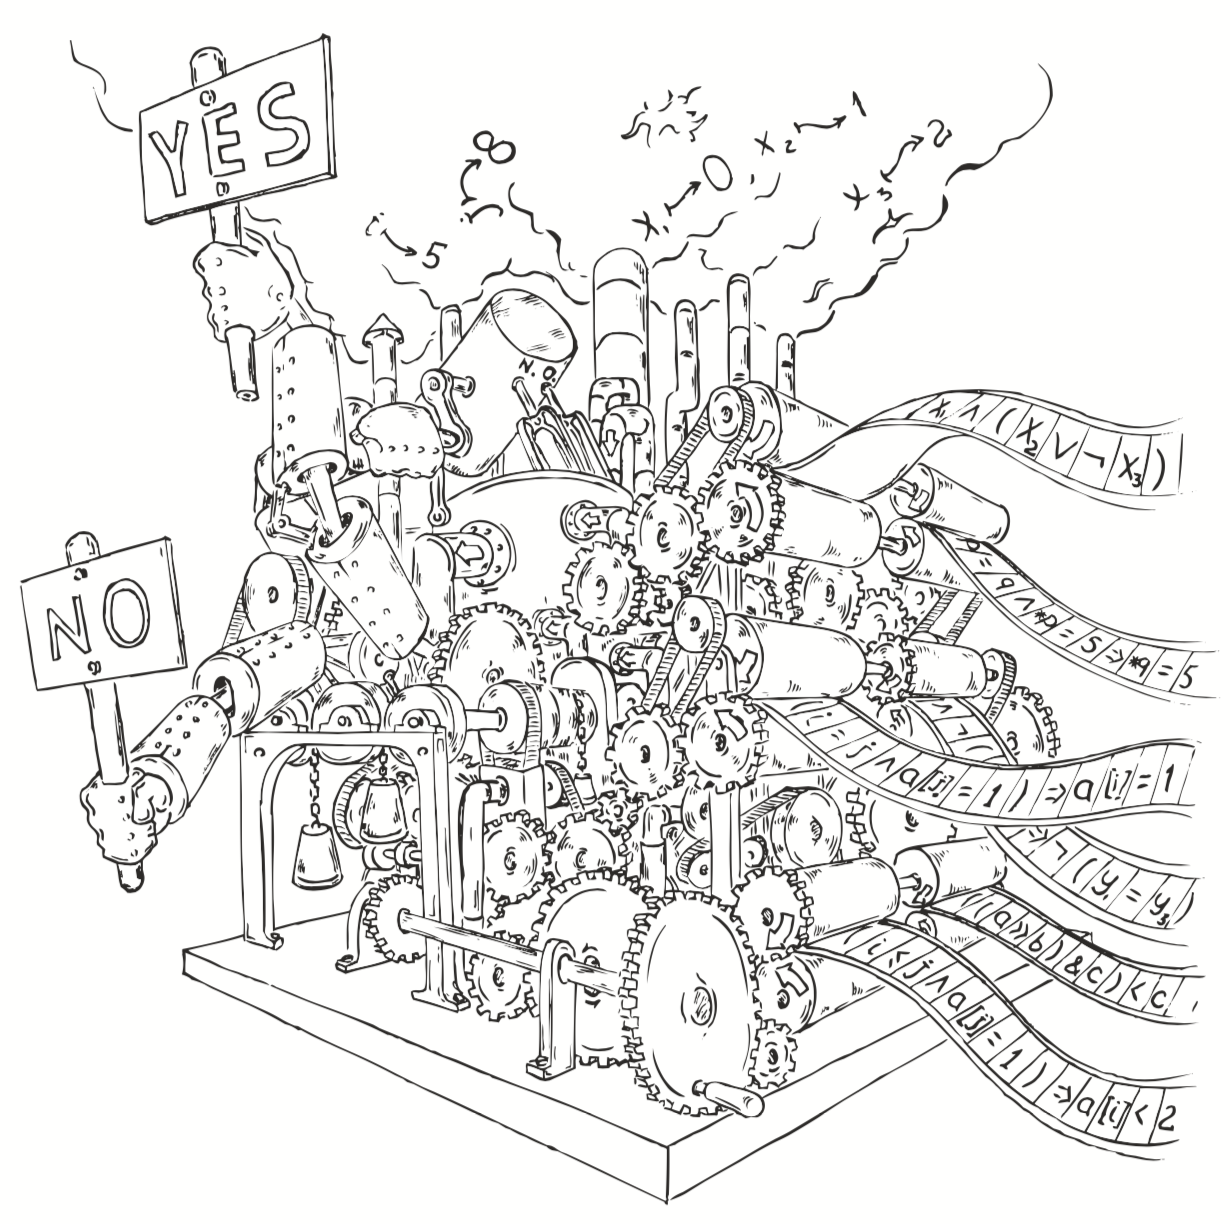
\includegraphics[scale=0.5]{../decision-procedure.png}
\end{frame}

\frame{\titlepage}

\begin{frame}{Два приминения EUF}
\begin{itemize}
\item Проверка процесса компиляции с помощью валидации трансляций
\end{itemize}
\end{frame}

\begin{frame}{Два приминения EUF}
\begin{itemize}
\item Доказательство эквивалентности двух схем
\item Проверка процесса компиляции с помощью валидации трансляций
\end{itemize}
\end{frame}

\begin{frame}{Логика линейной арифметики}
$formula: formula \vee formula | \lnot formula | (formula) | atom$\newline
$atom: sum op sum$\newline
$op: = | \le | <$\newline
$sum: term|sum + term$\newline
$term: identifier | constant | constant identifier$\newline
\end{frame}

\begin{frame}{Логика линейной арифметики}
$formula: formula \vee formula | \lnot formula | (formula) | atom$\newline
$atom: sum op sum$\newline
$op: = | \le | <$\newline
$sum: term|sum + term$\newline
$term: identifier | constant | constant identifier$\newline
$2z_1 + 3z_2 \le 5 \wedge z_2 + 5z_2 - 10z_3 \ge 6 \wedge z1 + z3 = 3$
\end{frame}

\begin{frame}{Логика линейной арифметики}
Пример: демо
\end{frame}

\begin{frame}{Домен}
\begin{itemize}
\item Рациональные числа
\end{itemize}
\end{frame}

\begin{frame}{Домен}
\begin{itemize}
\item Рациональные числа
\item Целые числа
\end{itemize}
\end{frame}

\begin{frame}{Рациональные числа}
\begin{itemize}
\item Существует полиномиальный алгоритм решения
\item Используется Симлекс метод, который в худшем случае экспоненциальный, но даёт хорошие результаты на реальных данных
\end{itemize}
\end{frame}

\begin{frame}{Целые числа}
\begin{itemize}
\item NP-трудная задача
\item Задача целочисленного линейного программирования
\end{itemize}
\end{frame}

\begin{frame}{Логика линейной арифметики}
$formula: formula \vee formula | \lnot formula | (formula) | atom$\newline
$atom: term rel term | Boolean-Identifier | term[constant]$\newline
$rel: = < | =$\newline
$term: term op term | identifier | ~term | constant | atom?term:term$\newline
$op: + | - | \times | / | << | >> | \& | | | \oplus | \circ$\newline
\end{frame}

\begin{frame}
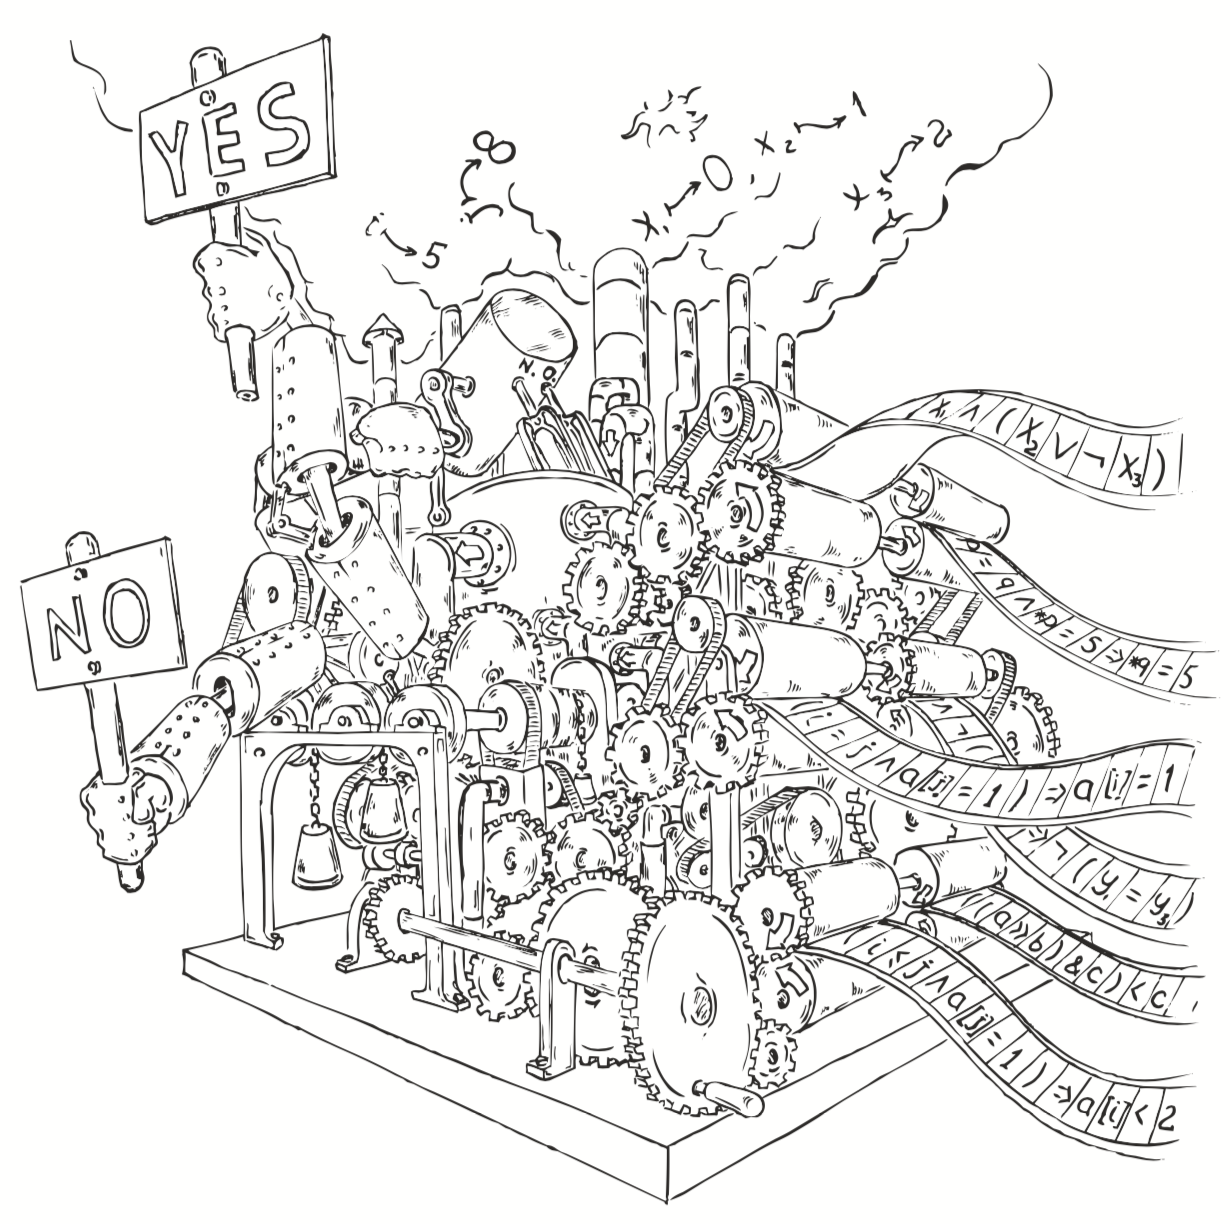
\includegraphics[scale=0.5]{../decision-procedure.png}
\end{frame}

\end{document}
